%\documentclass[12pt,a4paper,onecolumn]{beamer}

\documentclass[10pt, xcolor=x11names]{beamer}
\usecolortheme{seagull}
\useoutertheme{infolines}
\usefonttheme[onlymath]{serif}
\setbeamertemplate{headline}[default]
\setbeamertemplate{navigation symbols}{}
\mode<beamer>{\setbeamertemplate{blocks}[rounded][shadow=true]}
\setbeamercovered{transparent}
\setbeamercolor{block body example}{fg=blue, bg=black!20}

\usepackage[utf8]{inputenc}
\usepackage[german]{babel}
\usepackage[]{csquotes}
\usepackage{amsmath}
\usepackage{tikz, wasysym}
\usepackage{graphicx}
\usetikzlibrary{automata,positioning}
\usepackage{hyperref}

%\usepackage{amsfonts}
%\usepackage{amssymb}
%\usepackage{makeidx}
%\usepackage{graphicx}


\usepackage{hyperref}
\author{Sven Fiergolla}
\title[Kleines Studienprojekt]{Eine universelle Turingmaschine mit zwei Zuständen/Symbolen}
\subtitle[short version]{Ein Paper von Claude E. Shannon}
\date{\today}
%\institute[Uni Trier]{Universität Trier}
%\logo{\includegraphics[scale=.25]{unilogo.pdf}}

\begin{document}
	\frame{\maketitle}
	\frame{\frametitle{Übersicht}
	\tableofcontents
	}
	
	\frame{\frametitle{Einführung}
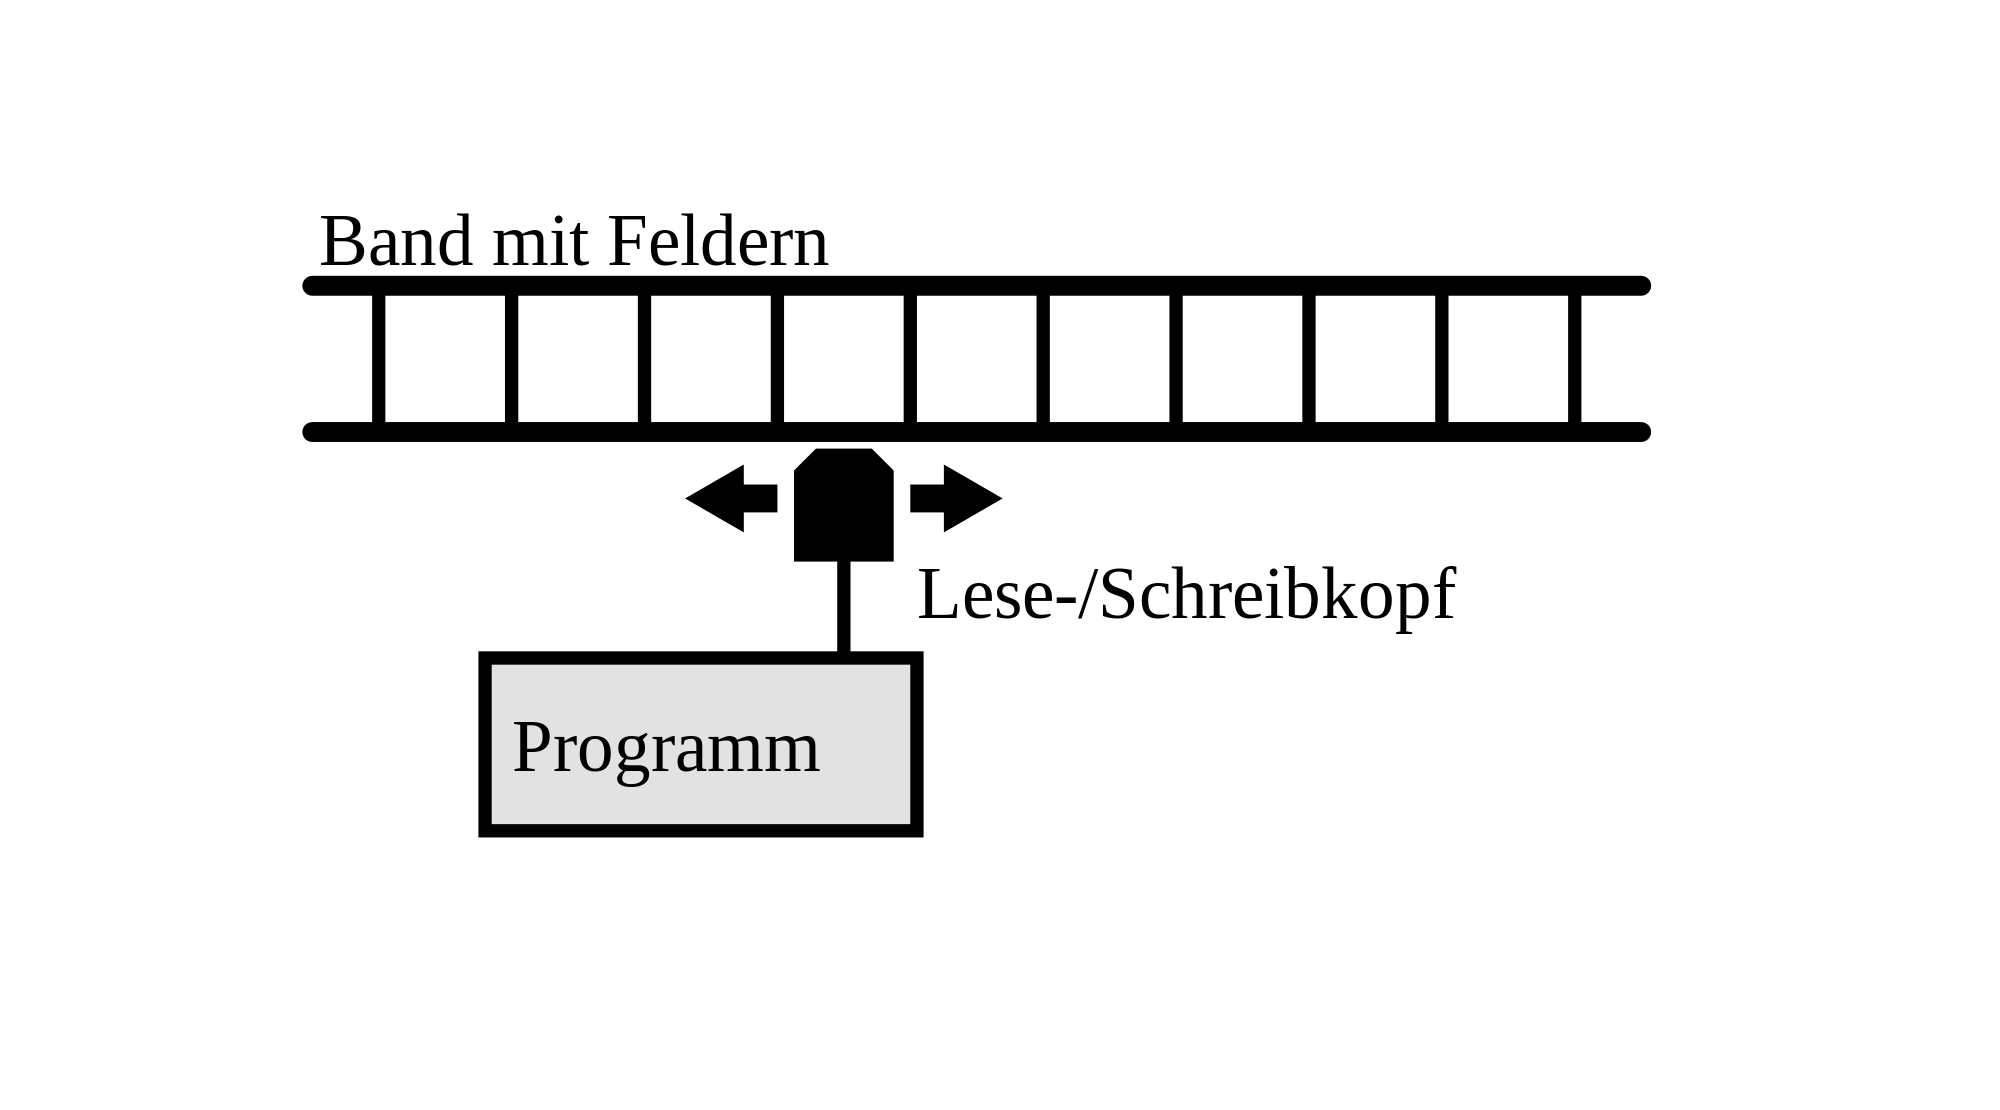
\includegraphics[scale=0.18]{2000px-Turingmaschine.png}
}


	\section{Einführung}
	\frame{\frametitle{Einführung}
Formal definieren wir die Turingmaschine als Sextupel $\mathbf{ M = (Q,\Sigma,\Gamma,q_0,\delta,\Square)} $
 wobei:

\begin{description}
 \item $\mathbf{ Q = }$ die endliche Zustandsmenge
 \item $\mathbf{ \Sigma = }$ das endliche Eingabealphabet
 \item $\mathbf{ \Gamma = }$ das endliche Bandalphabet und es gilt $\mathbf{\Sigma\subset\Gamma}$
 \item $\mathbf{ q_0 = }$ der Anfangszustand
 \item $\mathbf{ \delta = }$ die (partielle) Überführungsfunktion
 \item $\mathbf{ \square = }$ steht für das leere Feld (Blank)
\end{description}	
}



	\section{Universelle Turingmaschinen}
	\frame{\frametitle{Universelle Turingmaschinen}
		Formal ist eine universelle Turingmaschine eine Maschine $UTM$, die eine Eingabe $w|x$ liest.\\
		\medskip
		 Das Wort $w$ ist hierbei die Beschreibung einer Turingmaschine $M_{w}$, die zu einer bestimmten Funktion mit Eingabe $x$ die Ausgabe berechnet. Die $UTM$ simuliert also das Verhalten von $M_{w}$ mit Hilfe der Funktionsbeschreibung $w$ und der Eingabe $x$.
	}
	
	
	\section{Turingaschine mit zwei Zuständen}
	\frame{\frametitle{Zustände}
	Die Zustände von Maschine $B$ werden $\alpha$ und $\beta$ heißen.\\
	\medskip
	Um die Information des aktuellen Zustands nach bearbeiten eines Symbols in der nächsten Zelle zur Verfügung zu haben, auch wenn die $TM$ $B$ nur zwei Zustände hat, wird diese in den Symbolen gespeichert (Index $n$) und über die sogenannte \textit{bouncing operation} in die nächste Zelle übertragen.
	}	
	
	
	\frame{\frametitle{Konstruktion}
	Turingmaschine $A$: $ A_1,A_2,...,A_m \in$ $\Sigma_A$ die Symbole und $q_1,q_2,...q_n \in Q_A$ die Zustände der Maschine.
	Maschine $B$ besitzt:
\begin{itemize}
	\pause \item elementare Symbolen von Maschine $A$:  $B_1,B_2,...,B_m \in \Sigma_B$
	\pause \item $m\cdot n \cdot 2 \cdot 2$ neue Symbole, welche Informationen über den Zustand und den Status der \textit{bouncing operation} speichern: $B_{m,n,x,y} \in \Sigma_B$
	\begin{itemize}
	\pause \item $m =$ Symbole von $A, |\Sigma_A|$
	\item $n =$ Zustände von $A, |Q_A|$
	\item $x = +$ oder $-$ ob der Zustand des letzten Feldes in dieses Feld übertragen wird oder aus diesem Feld stammt 
	\item $y = R$ oder $L$  ob die Information in das rechte oder linke Feld übertragen wird.
	 
	\end{itemize}
\end{itemize}	
	 
	\pause Insgesammt besitzt Maschine $B$ also $m+4mn$ Symbole.  
	}
	

	
	\frame{\frametitle{Übergänge}
	\begin{center}
	\begin{tabular}{c c|c||c|c|c}

\textbf{Nr.}&\textbf{Symbol} & \textbf{Zustand $\Rightarrow$} & \textbf{Symbol} & \textbf{Zustand} &\textbf{Richtung} \\
\hline
(1) & $B_i$ & $\alpha$  & $B_{i,1,-,R}$  & $\alpha$ & $R$\\
\hline
(2) & $B_i$ & $\beta$  & $B_{i,1,-,L}$  & $\alpha$ & $L$\\
\hline
(3) & $B_{i,j,-,x}$ & $\alpha$ oder $\beta$  & $B_{i,(j+1),-,x}$  & $\alpha$ & $x\in \{ R,L \}$\\
\hline
(4) & $B_{i,j,+,x}$ & $\alpha$ oder $\beta$  & $B_{i,(j-1),+,x}$  & $\beta$ & $x\in \{ R,L \}$\\
\hline
(5) & $B_{i,1,+,x}$ & $\alpha$ oder $\beta$  & $B_i$  & $\alpha$ & $x\in \{ R,L \}$\\


\end{tabular}
\\
\bigskip
zusätzlich erhält Maschine $B$ für jeden Übergang in $A :$\\
\bigskip
(6) $\delta(A_i,q_j) \to (A_k,q_l,{R \atop L}) \Rightarrow \delta(B_{i,j,-,x},\alpha) \to (B_{k,l,+,{R \atop L} },{\beta \atop \alpha},{R \atop L})$\\


\end{center}
}
\section{Beispiel}
	\frame{\frametitle{Beispiel Maschine $A$}
	\begin{center}
	
	
	Maschine $A$:\\
	\bigskip
	$...|\underbrace{A_3}|A_{13}|...$
	
	\bigskip
		\begin{tikzpicture}[shorten >=1pt,node distance=3cm,on grid,auto]
   
   \node[state] (1)  {$q_7$};
   \node[state] (2) [right=of 1] {$q_4$};
   

   \path[->]
    (1) edge                    node {$A_3\:A_8\:R$} (2);

\end{tikzpicture}



\bigskip
$...|A_8|\underbrace{A_{13}}|...$
\end{center}
	}
	
	
	%TODO: nach und nach einblenden
	\frame{\frametitle{Beispiel Maschine $B$}
	\begin{tabular}{c||c c}
	\textbf{Bandinhalt} & \textbf{Übergangsfunktion} & \textbf{Gleichung}\\ \hline
	\\
	$...|\underbrace{B_{3,7,-,x}}|B_{13}|...$ &
	$\delta(B_{3,7,-,x},\alpha) = (B_{8,4,+,R},\beta,R)$ &  $(6)$\\ 
	\hline
	\pause $...|B_{8,4,+,R}|\underbrace{B_{13}}|...$ & $\delta(B_{13},\beta) = (B_{13,1,-,L},\alpha,L)$ & $(2)$\\
	\hline
	\pause $...|\underbrace{B_{8,4,+,R}}|B_{13,1,-,L}|...$ & $\delta(B_{8,4,+,R},\alpha) = (B_{8,3,+,R},\beta,R)$ & $(4)$\\
	\hline
	\pause $...|B_{8,3,+,R}|\underbrace{B_{13,1,-,L}}|...$ &$\delta(B_{13,1,-,L},\beta) = (B_{13,2,-,L},\alpha,L)$  & $(3)$\\
	\hline
	\pause $...|\underbrace{B_{8,3,+,R}}|B_{13,2,-,L}|...$ & $\delta(B_{8,3,+,R},\alpha) = (B_{8,2,+,R},\beta,R)$ & $(4)$\\
	\hline
	\pause $...|B_{8,2,+,R}|\underbrace{B_{13,2,-,L}}|...$ & $\delta(B_{13,2,-,L},\beta) = (B_{13,3,-,L},\alpha,L)$ & $(3)$\\
	\hline
	\pause $...|\underbrace{B_{8,2,+,R}}|B_{13,3,-,L}|...$ & $\delta(B_{8,2,+,R},\alpha) = (B_{8,1,+,R},\beta,R)$ & $(4)$\\
	\hline
	\pause $...|B_{8,1,+,R}|\underbrace{B_{13,3,-,L}}|...$ & $\delta(B_{13,3,-,L},\beta) = (B_{13,4,-,L},\alpha,L)$ & $(3)$\\
	\hline
	\pause $...|\underbrace{B_{8,1,+,R}}|B_{13,4,-,L}|...$ & $\delta(B_{8,1,+,R},\alpha) = (B_{8},\alpha,R)$ & $(5)$\\
	\hline
	\pause $...|B_{8}|\underbrace{B_{13,4,-,L}}|B_{x}|...$ & $\dots$ & $(6)$\\
	\end{tabular}
	}
	
	\section{Unmöglichkeit einer universellen Turingmaschine mit einem Zustand}
	\frame{\frametitle{$UTM$ mit nur einem Zustand unmöglich}
	Beweis per Kontraposition von Shannon:\\
	Annahme: es existiert eine universelle Turingmaschine mit nur einem Zustand.\\
	
		\bigskip
	\pause $\sqrt{2}$ ist eine berechenbare irrationale Zahl und kann von einer $UTM$ berechnet werden. Dazu muss die $UTM$ kontinuierlich die Ziffern von $\sqrt{2}$ schreiben.
	
	\bigskip
	\pause $\sqrt{2}$ ist turingberechenbar $\Rightarrow$ eine $UTM$ kann $\sqrt{2}$ berechnen
	

	}
	
	
	\frame{\frametitle{$\sqrt{2}$ mit nur einem Zustand berechnen}
	Annahme: doppelt unendliches Band
	\begin{itemize}
	\visible<2->{ \item $1.1:$ Lesekopf liest $\Square$ und bleibt im $\Square$-Bereich}
	\visible<3->{\item $1.2:$ Lesekopf verlässt $\Square$}
	\begin{itemize}
	\visible<4->{\item $1.2.1:$ Lesekopf verlässt $\Square$ nach links}
	\begin{itemize}
	\visible<5->{\item $1.2.1.1$ linke unendliche Seite des Bandes wird nicht betreten}
	\visible<6->{\item $1.2.1.2$ linke unendliche Seite des Bandes wird betreten}
	\end{itemize}
	\visible<7->{\item $1.2.2:$ Lesekopf verlässt $\Square$ nach Rechts}
	\end{itemize}
	\end{itemize}

	%1.1
	\only<2>{$1.1$ Die $TM$ wird nie mehr als ein $\Square$ der Eingabe verändern $\Rightarrow$ das Eingabeband ist nur auf einem endlichen Teil beschrieben $\Rightarrow$ das Band kann nach der Bearbeitung nicht $\sqrt{2}$ enthalten.}
	
	\only<5>{$1.2.1.1$ Die $TM$ betritt nur eine Seite des Bandes $\rightarrow$ wird in Fall $2$ behandelt}
	
	\only<6>{$1.2.1.2$ Die $TM$ geht unendlich weit nach Links $\Rightarrow$ linke Seite des Bandes wird mit konstantem Symbol beschrieben und rechte unendliche Seite des Bandes nie betreten $\Rightarrow$ Band kann nach der Bearbeitung nicht $\sqrt{2}$ enthalten.}
	
	\only<7>{$1.2.2$ analog zu $1.2.1$.\\
	Damit können wir annehmen, dass das Band nur einseitung unendlich ist (Band ist rechts der Eingabe unendlich)}
	}
	
	\frame{\frametitle{\textit{reflection number} $R$ der Maschine}
	Beweishilfe: \enquote{\textit{reflection number}}\\
	platziere den Lesekopf auf dem ersten $\Square$ nach der Eingabe:\\
	\begin{itemize}
	\item Lesekopf wird sich evtl. zur Eingabe hin bewegen
	\pause \item $||...|1|0|\underbrace{\Square}|\Square$ $\rightarrow$ 
	$||...|1|\underbrace{0}|x|\Square$
	\end{itemize}
	\pause wenn der Lesekopf die Eingabe betritt, platziere ihn wieder auf dem selben Feld.\\ 
	\begin{itemize}
	\item $||...|1|0|\underbrace{x}|\Square$
	\end{itemize}
	\bigskip
	wie oft man die Lesekopf so platzieren kann, nennt man \textit{reflection number}, $R \in N$
	}
	
	\frame{\frametitle{\textit{reflection number} $S$ für die Eingabe $\sqrt{2}$}
	
	platziere den Lesekopf am Anfang der Eingabe
	\begin{itemize}
	\item $||\underbrace{A_1}|A_2|...|A_m|\Square|\Square|...$
	\end{itemize}
	
	der Lesekopf wird die Eingabe verlassen
	\begin{itemize}
	\pause \item $||A_1|A_2|...|A_m|\underbrace{\Square}|\Square|...$
	\end{itemize}	 
	
	platziere den Lesekopf am Ende der Eingabe
	\begin{itemize}
	\pause \item $||A_1|A_2|...|\underbrace{A_m}|A_x|\Square|\Square|...$
	\end{itemize}
	der Lesekopf wird sich evtl. wieder von der Eingabe weg bewegen.\\
	\bigskip	
	wie oft man die Lesekopf so platzieren kann, nennen wir die \textit{reflection number} für $\sqrt{2} =:S$ 
	}
	

	
	%TODO : Fälle abklären!	
	
		\frame{\frametitle{$\sqrt{2}$ mit nur einem Zustand berechnen}
	Annahme: einseitig unendliches Band\\

	\begin{itemize}
	\item $2.1$ $S<\infty$ und $S < R$
	\visible<2->{\item $2.2$ $S=R=\infty$}
	\begin{itemize}
	\visible<3->{\item $2.2.1$ Lesekopf betritt nur endlichen Bereich des Bandes}
	\visible<4->{\item $2.2.2$ Lesekopf betritt unbeschränkten Bereich des Bandes}
	\begin{itemize}
	\visible<5->{\item $2.2.2.1$ Symbol in allen Zellen konstant}
	\visible<6->{\item $2.2.2.2$ Symbole in den Zellen ändern sich endlos}
	\end{itemize}
	\end{itemize}
	\visible<7->{\item $2.3$ $R \leq S$ ($R$ endlich)}
	\begin{itemize}
	\visible<9->{\item $2.3.1$ $k \leq R \leq S$}
	\visible<10->{\item $2.3.2$ $k > R$}	
	\end{itemize}
	\end{itemize}

	\only<1>{$2.1$ nach einer endlichen Anzahl an Schritten ist der Lesekopf im Bereich der Eingabe \enquote{gefangen} $\Rightarrow$ Band ist nur auf endlichem Teil beschrieben. $\Rightarrow$ Band kann nicht $\sqrt{2}$ enthalten.}
	\only<2>{$2.2$ Der Lesekopf kommt unendlich oft wieder zur Eingabe zurück. Der urprünglich leere Bereich des Bandes wird entweder beschränkt oder unbeschränkt weit beschrieben.}
	\only<3>{$2.2.1$ nur endlicher Teil des Bandes beschrieben $\Rightarrow$ Band kann nicht $\sqrt{2}$ enthalten}
	\only<4>{$2.2.2$ unbeschränkter Teil des Bandes wird betreten\\
	Da die $TM$ nur über ein endliches Alphabet verfügt und nur einen Zustand hat, muss dass Symbol entweder in allen Zellen Konstant sein oder sich ständig ändern.}
	\only<5>{$2.2.2.1$ Symbole in allen Zellen konstant $\Rightarrow$ kann nicht $\sqrt{2}$ beschreiben}
	\only<6>{$2.2.2.2$ Symbole in allen Zellen ändern sich endlos $\Rightarrow$ kann nicht $\sqrt{2}$ beschreiben}
	\only<7-11>{$2.3$ Lesekopf betritt ursprünglich unbeschriebenen Bereich des Bandes und bleibt dort\\}
	\only<8-11>{$k:=$ Anzahl wie oft Lesekopf das erste ursprünglich leere Feld nach rechts verlässt}
	
	\only<9>{$2.3.1$ $k \leq R \leq S \Rightarrow$  Lesekopf auf erstem $\Square$ gefangen}
	
	\only<10-11>{$2.3.2$ $k > R$\\
	erstes ursprünglich leeres Feld wird $2R$ mal besucht (enthält Beschriftung welche der Lesekopf auf ein $\Square$ nach $2R$ Schritten schreibt)}
	\only<11>{gilt für das nächste und für alle folgenden ursprünglich unbeschrifteten Felder $\Rightarrow$ Band enthält konstante Beschriftung}
	
	%TODO 	
%	\only<8>{$2.3.1$ Lesekopf verlässt erstes leere Feld nach Links\\
%	Band wird mit konstantem Symbol beschrieben $\Rightarrow$ Band kann nicht $\sqrt{2}$ %enthalten}
%	\only<9>{$2.3.2$ Lesekopf verlässt erstes leeres Feld $R$ mal nach rechts $\Rightarrow$ Lesekopf wird nicht zu erstem leeren Feld zurückkommen, da $R$ die \textit{reflection number} für $\Square$ ist}
%	\only<10>{$2.3.2.1$ Lesekopf auf erstem $\Square$ gefangen $\Rightarrow$ Band enthält nicht $\sqrt{2}$}
%	\only<11>{$2.3.2.2$ Lesekopf verlässt erstes $\Square$ $R$-mal, ($R=$ \textit{reflection number für $\Square$}) $\Rightarrow$ Lesekopf wird nicht zum ersten leeren Feld zurückkehren $\Rightarrow$ diese Feld enthält das Ergebniss eines $\Square$-Feldes das $2\cdot R$ mal besucht wurde. Das nächste Feld jedoch auch, da die Maschine auf einer endlosen Folge von $\Square$ arbeitet $\Rightarrow$ alle Felder enthalten konstantes Symbol.} 
	
	}
	
	\section{Aquivalente Turingmaschine mit nur zwei Symbolen}
	\frame{\frametitle{äquivalente TM mit nur zwei Symbolen}

	Turingmaschine $A$: $ A_1,A_2,...,A_m \in$ $\Sigma_A$ die Symbole und $q_1,q_2,...q_n \in Q_A$ die Zustände der Maschine.
	Maschine $C$ besitzt:
\begin{itemize}
	\item die Symbole $\{\Square,1\} \in \Sigma_B$
\end{itemize}
	\pause Zudem sei $l$ Imfimum für $ m\leq 2^l$ \\
	Nun können Symbole der Maschine $A$ als Binärsequenzen der Länge $l$ interpretiert werden. zB.: $\Square_A \equiv \Square_C^l$
	\begin{itemize}
	\item für Maschine $C$ gilt $|Q_C| \leq 3n 2^l + n(2^l -7)$ 
	\end{itemize}
	 }
	 
	 
	 
	 	\frame{\frametitle{Beispiel Maschine $A$}
	\begin{center}
	
	
	Maschine $A$:\\
	\bigskip
	$...|\underbrace{A_3}|A_{13}|...$
	
	\bigskip
		\begin{tikzpicture}[shorten >=1pt,node distance=3cm,on grid,auto]
   
   \node[state] (1)  {$q_7$};
   \node[state] (2) [right=of 1] {$q_4$};
   

   \path[->]
    (1) edge                    node {$A_3\:A_8\:R$} (2);

\end{tikzpicture}



\bigskip
$...|A_8|\underbrace{A_{13}}|...$
\end{center}
	}
	\frame{\frametitle{Beispiel Maschine $C$}
	\begin{center}
	  Maschine $C$ ist in Zustand $T_3$\\

\bigskip
	
	\only<1>{$...|\overbrace{\underbrace{1}|1|\Square|1|\Square|...}^{\text{Binärkodierung von A3}}|1|\Square|...$}
		\only<2>{$...|\overbrace{1|\underbrace{1}|\Square|1|\Square|...}^{\text{l Felder lang}}|1|\Square|...$}
		\only<3>{$...|\overbrace{1|1|\underbrace{\Square}|1|\Square|...}^{\text{l Felder lang}}|1|\Square|...$}
		
 
 
	\end{center}
	\bigskip
 
 		\begin{tikzpicture}[shorten >=1pt,node distance=3cm,on grid,auto]
   
   \node[state] (1) at (0,0) {$T_3$};
   
   \only<1>{
   \node[state] (2) at (2,1) {$T_{3,1}$};
   \node[state] (3) at (2,-1) {$T_{3,0}$};
   }
   
   \only<2>{
   \node[state] (2) at (2,0) {$T_{3,1}$};
   \node[state] (3) at (4,1) {$T_{3,1,1}$};
   \node[state] (4) at (4,-1) {$T_{3,1,0}$};
   }
   
      \only<3>{
   \node[state] (2) at (2,0) {$T_{3,1}$};
   \node[state] (3) at (4,0) {$T_{3,1,1}$};
   \node[state] (4) at (6.5,1) {$T_{3,1,1,1}$};
   \node[state] (5) at (6.5,-1) {$T_{3,1,1,0}$};
   }
   


    \only<1>{
       \path[->]
    (1) edge    node[above, yshift=0.4cm] {$1\:1\:R$} (2)
    (1) edge    node[below, yshift=-0.4cm] {$\Square\:\Square\:R$} (3);
    }
    
        \only<2>{
           \path[->]
    (1) edge    node[above] {$1\:1\:R$} (2)
    (2) edge    node[above, yshift=0.4cm] {$1\:1\:R$} (3)
    (2) edge    node[below, yshift=-0.4cm] {$\Square\:\Square\:R$} (4);
    }
 
 
        \only<3>{
           \path[->]
    (1) edge    node[above] {$1\:1\:R$} (2)
    (2) edge    node[above] {$1\:1\:R$} (3)
    (3) edge    node[above, yshift=0.4cm] {$1\:1\:R$} (4)
    (3) edge    node[below, yshift=-0.4cm] {$\Square\:\Square\:R$} (5);
    }
    
\end{tikzpicture}

	}
	
		\frame{\frametitle{äquivalente TM mit nur zwei Symbolen}

	Turingmaschine $C$ nutzt also $(2^l-1)\cdot n$ Zustände $T_i,T_{i,1},T_{i,0},T_{i,1,1}...$ um die aktuellen Informationen über die Zustand und das gelesene Zeichen zu halten. \pause Nach $l$ eingelesenen Symbolen hat $TM$ $C$ ein Symbol der Maschine $A$ gelesen und befindet sich in Zustand $T_{i,x_1,x_2,x_3,...x_{l-1}}$\\
	\bigskip
	Die jetzt angewendete Übergangsfunktion hängt direkt von Maschine $A$ ab.\\
	\begin{center}
	$\delta(A_i,q_j) \to (A_k,q_l,{R \atop L})$\\
	$\Rightarrow $ \\
	$\delta(\{1\text{ oder } \Square \},T_{i,x_1,x_2,...x_{l-1}}) \to (\{1\text{ oder } \Square \},{R_{i,y_1,y_2,...y_{l-1}} \atop L_{i,y_1,y_2,...y_{l-1}}},{L \atop R})$	
	\end{center}
	 }
	 
	 	\frame{\frametitle{äquivalente TM mit nur zwei Symbolen}
	 	Für die Ausgabe gibt es $R_{i,y_1,y_2,...y_{l-1}} \atop L_{i,y_1,y_2,...y_{l-1}}$ Zustände welche Binärkodierung des zu schreibenden Symbols in die einzelnen Felder ausgibt.\\
	 	\bigskip
	 	Anschließend muss der Lesekopf auf die richtige Position bewegt werden.
	 	
	 	\begin{center}
	 	$...|\overbrace{\underbrace{1}|1|\Square|1|\Square|...}^{\text{l Felder lang}}|1|\Square|... \ \ \rightarrow \ \	...|\overbrace{1|1|\Square|1|\Square|...}^{\text{l Felder lang}}|\underbrace{1}|\Square|...$
	 	\end{center}
	 	
	 	Dafür existieren $2n(2^l-2)$ $R$ bzw. $L$-Zustände sowie $2n(2^l-1)$ $U$ bzw. $V$-Zustände, die den Lesekopf nach dem Schreiben einer Zeichenkette, $l$ Positionen nach Links oder Rechts bewegegen.

	 }
	 
	 \section{Fazit}
	 \frame{\frametitle{Fazit}
	 Informationen lassen sich innerhalb bestimmter Grenzen, in Zustände bzw. Symbole einer $TM$ auslagern.\\
	 Bei der Konstruktion der $TM$ mit nur 2 Zuständen stieg das Produkt des Modells um den Faktor 8, bei der Konstruktion mit 2 Symbolen um einen Faktor von ca. 6.\\
	 \bigskip
	 \pause Diesen Verlust erklärt Shannon durch die Art der Konstruktion und dass sich die Faktoren bei performanterer Modellierung nahezu angleichen. 
	 }
	 
	 	 \frame{\frametitle{Fazit}
	Shannon endet das Paper mit der Fragestellung:\\
	 \enquote{An interesting unsolved problem is to find the minimum possible state-symbol product for a universal Turing machine}\\
	 \bigskip
	 \begin{itemize}
	 \pause \item Wolfram Alpha versprach ein Preisgeld von 25,000 für den Beweis der Universalität einer (2,3) Turingmachine. (2 Zustände, 3 Symbole)
	 \item Am 24 October 2007 wurde bekanntgegeben, dass Alex Smith, Student an der University of Birmingham, die Universalität der (2,3) TM bewiesen hat.
	 \end{itemize}
	 
	 }
	 
	 \section{Quellen}
	 	 \frame{\frametitle{Quellen}
	
	\begin{itemize}
		\item Shannon, C. E. \enquote{A Universal Turing Machine with Two Internal States.} Automata Studies. Princeton, NJ: Princeton University Press, pp. 157-165, 1956. \footnote{\url{http://www.sns.ias.edu/~tlusty/courses/InfoInBio/Papers/Shannon1956.pdf}}
		\item Wolfram Research and Wolfram, S. \enquote{The Wolfram 2,3 Turing Machine Research Prize.} \footnote{\url{http://www.wolframscience.com/prizes/tm23/}}
		\item Wolfram, S. A New Kind of Science. Champaign, IL: Wolfram Media, pp. 706-711 and 1119, 2002.
	\end{itemize}
	 
	 }
	
	
	
\end{document}
